\documentclass{article}
\usepackage[utf8]{inputenc}
\usepackage[spanish]{babel}
\usepackage{lmodern}
\renewcommand*{\familydefault}{\sfdefault}
\usepackage{graphicx}
\usepackage{titling}
\usepackage{geometry}
\usepackage{setspace}
\usepackage{tikz}
\usepackage{eso-pic}
\usepackage{ragged2e}
\usepackage{hyperref}
\usetikzlibrary{calc}
\usepackage{fancyhdr}
\usepackage{float}
\usepackage{amsmath}

\geometry{
    a4paper,
    total={170mm,257mm},
    left=2.05cm,
    top=3.5cm,
    bottom=30mm,
}

\newcommand{\vcentered}[1]{\begingroup\setbox0=\hbox{#1}
    \parbox{\wd0}{\box0}\endgroup}

% Borde de página
\AddToShipoutPictureBG{
    \begin{tikzpicture}[remember picture,overlay]
        \draw[line width=1pt] ($(current page.north west) + (1cm,-1cm)$) rectangle ($(current page.south east) + (-1cm,1cm)$);
    \end{tikzpicture}}

\begin{document}
    \begin{titlepage}
        \begin{picture}(0,0)
            \put(-20,-70){
\includegraphics[scale=.1]{ipn.png}}
        \end{picture}
        \begin{picture}(0,0)
            \put(320,-50){
\includegraphics[scale=.5]{escom.png}}
        \end{picture}
        \vspace{3cm}
        \begin{spacing}{2}
        \begin{center}
            {\huge \textit{\textbf{Instituto Politécnico Nacional \\ 
                        Escuela Superior de Cómputo \\ 
                        Profesor:  \\  Andres Garcia Floriano \\
                        Alumno: \\ Hernández Jiménez Erick Yael \\ Patiño Flores Samuel \\ Robert Garayzar Arturo \\ 
                        5BV1 \\ 
                        Practica:  \\ SMOTE y Perceptrón Simple }}}
        \end{center}
        \end{spacing}       
    \end{titlepage}
    
    %Pie de página
    \pagestyle{fancy}
    \fancyhf{}
    \fancyfoot[C]{\thepage} 
    \renewcommand{\headrulewidth}{0pt} 
    \newpage
    \tableofcontents
    \newpage
    \section{Introducción}
    \subsection{SMOTE}
    El \textbf{SMOTE} (Synthetic Minority Over-sampling Technique) es una técnica de sobremuestreo ampliamente utilizada en el ámbito del aprendizaje automático para abordar el problema del desequilibrio de clases en conjuntos de datos de clasificación. Este desbalance ocurre cuando una de las clases está representada de manera considerablemente menor en comparación con las demás, lo que puede sesgar el desempeño de los modelos predictivos hacia la clase mayoritaria, resultando en un rendimiento deficiente al identificar correctamente instancias de la clase minoritaria.

    La técnica SMOTE se diferencia de métodos más simples, como la replicación de instancias, al generar nuevos ejemplos sintéticos en lugar de duplicar observaciones existentes. Para ello, selecciona un punto de la clase minoritaria y, a partir de sus vecinos más cercanos, crea ejemplos sintéticos interpolando valores en el espacio de características. De esta manera, SMOTE expande de manera más robusta el espacio ocupado por la clase minoritaria, mejorando la representatividad de esta en el conjunto de datos y reduciendo el sesgo hacia la clase mayoritaria.
    
    El uso de SMOTE es común en tareas de clasificación donde el equilibrio entre las clases resulta crítico para la precisión global del modelo, como en la detección de fraudes, el diagnóstico médico y otras áreas donde la identificación precisa de clases raras o menos representadas puede ser crucial.
    
\subsection{Perceptrón Simple}

El \textbf{Perceptrón simple} es uno de los modelos fundamentales en el campo del aprendizaje automático y representa una de las primeras formas de redes neuronales artificiales. Desarrollado por Frank Rosenblatt a finales de la década de 1950, el perceptrón simple constituye un clasificador binario que, mediante una combinación lineal de entradas ponderadas, busca establecer un límite de decisión para separar dos clases.

Este modelo se basa en un proceso de aprendizaje supervisado en el que ajusta sus pesos internos mediante un algoritmo de retroalimentación, generalmente basado en la regla delta. Cada entrada del perceptrón se multiplica por un peso, se suma un sesgo (o término de polarización) y el resultado se pasa a través de una función de activación, que usualmente es una función escalón. Si el resultado excede un umbral determinado, se clasifica en una clase; de lo contrario, en la otra.

El perceptrón simple es capaz de resolver únicamente problemas linealmente separables, lo que implica que los datos deben poder dividirse mediante una línea (o un hiperplano en dimensiones superiores). Esta limitación, señalada por Minsky y Papert en su libro Perceptrons (1969), motivó el desarrollo de arquitecturas de redes más complejas, capaces de manejar problemas no linealmente separables, como las redes neuronales multicapa.

A pesar de su simplicidad, el perceptrón simple sentó las bases para el desarrollo de modelos más avanzados de aprendizaje profundo y se reconoce como un paso crucial en la evolución de la inteligencia artificial y la teoría de redes neuronales.

\section{Técnicas de separación de dataset}

\subsubsection{Validación Leave-One-Out (LOO)}

La \textbf{validación Leave-One-Out (LOO)} es un caso particular de validación cruzada en el que el número de subconjuntos es igual al número de observaciones en el conjunto de datos. En cada iteración, se utiliza una única observación como conjunto de prueba y el resto de las observaciones como conjunto de entrenamiento. Esto se repite tantas veces como observaciones haya, lo que da lugar a evaluaciones altamente exhaustivas. Aunque ofrece una estimación imparcial del error de generalización, LOO puede ser computacionalmente costoso para conjuntos de datos grandes debido a la gran cantidad de particiones.

\subsubsection{n-fold Cross-Validation}

La \textbf{validación cruzada de n-fold} implica dividir el conjunto de datos en \(n\) subconjuntos (o `folds') de aproximadamente el mismo tamaño. En cada iteración, uno de estos subconjuntos se utiliza como conjunto de prueba y el resto como conjunto de entrenamiento. Este proceso se repite \(n\) veces, con cada subconjunto utilizado como conjunto de prueba una vez. El rendimiento se evalúa promediando las métricas obtenidas en cada iteración. Este método proporciona un equilibrio entre la cantidad de datos de entrenamiento disponibles y el tiempo computacional, y su versión más común es la \textit{10-fold cross-validation}.

\section{Comparativa}
SMOTE mejora el equilibrio de clases, lo que a menudo resulta en mejores métricas de rendimiento para clasificadores; fácil de implementar. Puede generar datos sintéticos no representativos o causar sobreajuste en casos extremos.

El perceptrón simple es rápido y eficiente para problemas linealmente separables; buena base para entender modelos de clasificación más complejos. No funciona bien con datos no linealmente separables o con problemas complejos de múltiples clases sin modificaciones.

El 1NN tiene la capacidad para clasificar conjuntos de datos con límites de decisión complejos; flexible y no requiere suposiciones sobre la distribución de los datos. Sufre en presencia de ruido, puede ser computacionalmente costoso con grandes conjuntos de datos, y sufre más cuando hay desequilibrio de clases si no se combina con técnicas como SMOTE

   
    \section{Desarrollo}
    
    Los resultados obtenidos son los siguientes: 

    \begin{figure}[!ht]
        \centering
        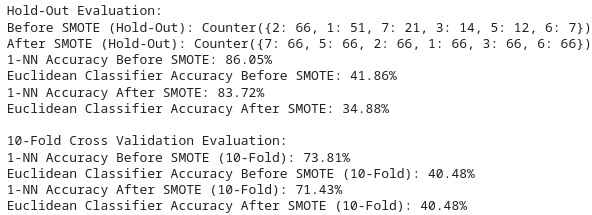
\includegraphics[scale=0.8]{Resultados_1.png}
        \caption{Resultados conjuntos obtenidos. Parte 1.}
    \end{figure}
    \newpage
    
    \begin{figure}[!ht]
        \centering
        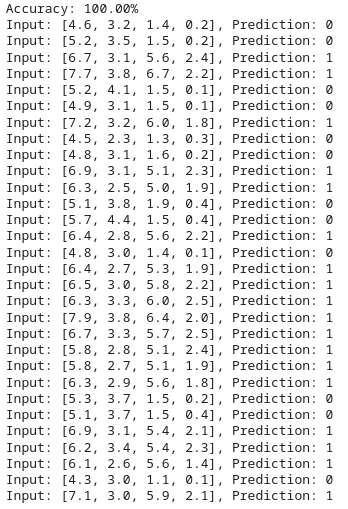
\includegraphics[scale=0.6]{Resultados_2.png}
        \caption{Resultados conjuntos. Parte 2.}
    \end{figure}
    
    % !TeX root = main.tex
\section{Conclusiones} 
    
\textbf{\Large Hernández Jiménez Erick Yael:}

Con los resultados anteriormente vistos, podemos notar la gran mejora en la precisión que nos otorga este modelo comparado con otros modelos implementados en prácticas anteriores y que, pese a su relativa simplicidad, la asunción que se hace de que las características se encuentran no relacionadas entre sí ayuda demasiado a no solo clasificar adecuadamente las clases, sino también encontrar más patrones entre sí.

\textbf{\Large Patiño Flores Samuel:}

Naive Bayes se distingue por la suposición de independencia entre las características, lo cual permite simplificar los cálculos de probabilidad. Aunque en muchos casos esta suposición no se cumple completamente, el modelo sigue mostrando buenos resultados en varias aplicaciones prácticas, como la clasificación de texto, detección de spam, y análisis de sentimientos. La simplicidad de Naive Bayes no solo lo hace computacionalmente eficiente, sino también fácil de interpretar, lo cual es una ventaja en situaciones donde la explicabilidad es importante.

\textbf{\Large Robert Garayzar Arturo:}

En esta práctica, implementamos y evaluamos el clasificador Naïve Bayes usando tres métodos de validación: Hold-Out estratificado, validación cruzada estratificada de 10 pliegues y Leave-One-Out. Esto permitió observar cómo varía el rendimiento del modelo en diferentes escenarios. El clasificador demostró ser efectivo, aunque su precisión depende de la estructura de cada conjunto de datos. Las métricas de Accuracy y la matriz de confusión brindaron una visión clara sobre el desempeño, confirmando que Naïve Bayes es una opción útil para tareas de clasificación básicas.
    
\end{document}
